\subsection{Networked Simulator}
\label{sec:netsim}
We implemented the networked simulator in its entirety in over 1100 sloc of Java (including all helper classes and interfaces, not including the rabinhash library). The software architecture can be seen in Figure \ref{fig:netsim_arch}. The networked simulator consists of the proxy server (\texttt{ProxyServerNet}) and the mobile client simulator (\texttt{SimulatorV3}), which is a wrapper for the networked mobile client (\texttt{MobileClientNet}) and is capable of performing several rounds of requests to the proxy server in real-time. It does so by prompting the user to manually enter the next web page URL she wishes to visit, simulating a web browser (see Figure \ref{fig:mobsim_ui} for an example of the user interface of our mobile client).

\begin{figure}[h] 
%\centering 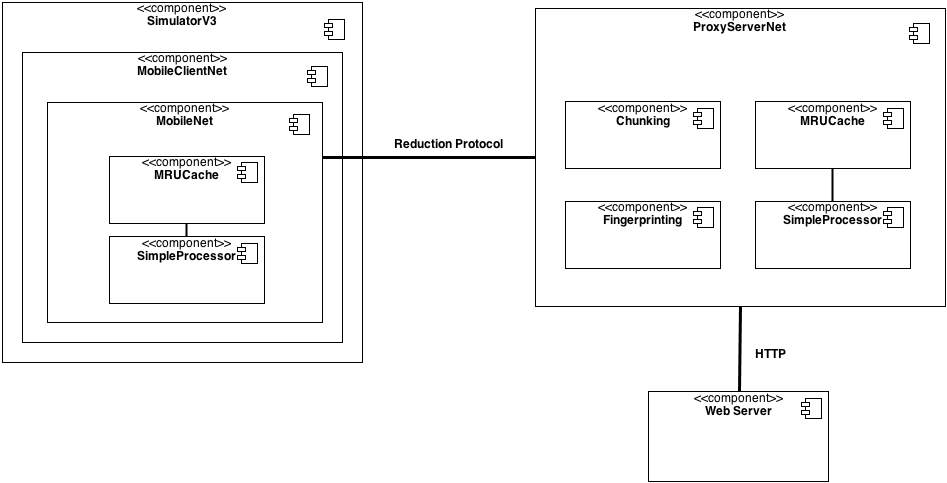
\includegraphics[scale=0.70]{diagrams/component_diagram.png}
\caption{Networked Simulator Software Architecture.}
\label{fig:netsim_arch}
\end{figure}

\begin{figure}[h] 
\centering 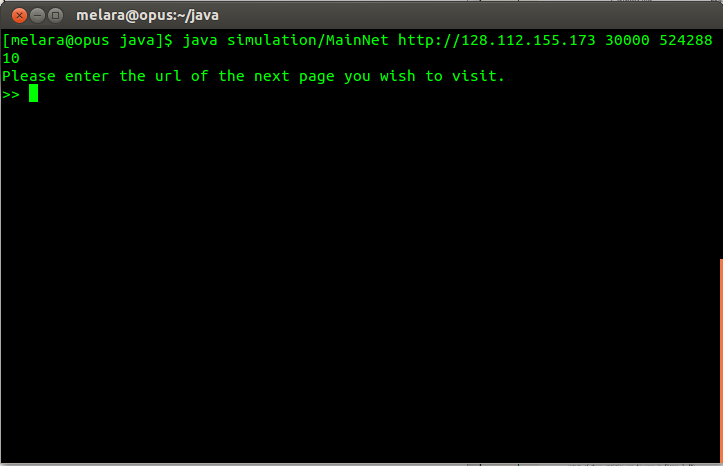
\includegraphics[scale=0.70]{images/mobilesim_ui.png}
\caption{The User Interface of our Mobile Client Simulator.}
\label{fig:mobsim_ui}
\end{figure}

In more detail, the networked simulator implements our reduction protocol as follows. First, the mobile client opens a socket to the proxy server, which is listening for connections at a user-specified port. The mobile client sends a simplified HTTP request of the format \emph{GET <url> HTTP/1.1} to the proxy server. It then formulates a proper HTTP request, including the User-Agent string of a mobile device\footnote{We use the Samsung Galaxy SII as our model mobile device across all our implementations and experiments.} to ensure that it receives the mobile version of the requested web page from the hosting web server. Once the proxy has received the content of the requested page from the appropriate web server, it engages in the reduction protocol\footnote{Minor changes were made to the chunking facility as well as the mobile device definition to support networking.} with the mobile client, exchanging the relevant information via the network. At the end, the mobile client reconstructs the content data of the received web page into an HTML file, which can then be viewed in any web browser. After the proxy has served the mobile client's request, the client is able to make a new request and repeat this process.

During each round of the protocol, both the proxy server and the mobile client simulator display three statistics to the user: (1) The number of chunks (and hence fingerprints) processed, (2) The remaining cache capacity after processing a web page, and (3) The cache missrate for the last web page processed. Moving towards our ultimate goal of reducing the required bandwidth for mobile phones to save data plan usage, we can use these statistics to calculate the average mobile cache missrate for one series of protocol simulations, as well as the average number of bytes transmitted between the proxy server and the mobile client. A sample simulator output of these statistics can be seen in Figure \ref{fig:mobsim_output}. We elaborate further on these calculations in Section \ref{sec:eval}.

\begin{figure}[h] 
\centering 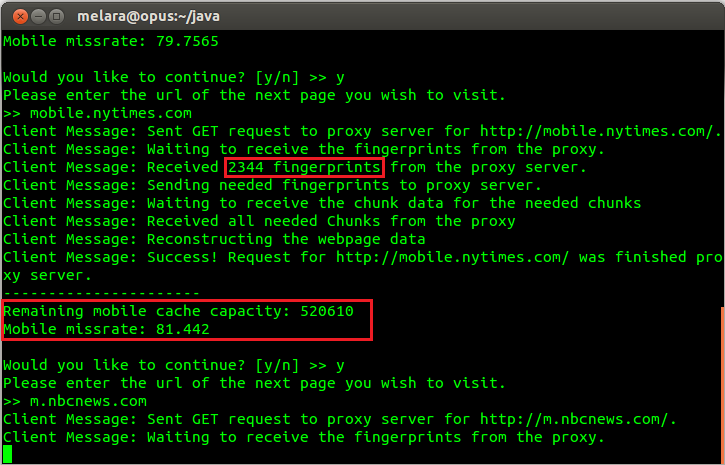
\includegraphics[scale=0.70]{images/mobilesim_output.png}
\caption{Sample Output of our Mobile Client Simulator.}
\label{fig:mobsim_output}
\end{figure}

We found that, while simulating mobile browsing, for one not using an actual mobile phone, and for another not using a web browser program of any sort, is not realistic, our networked simulator is a good first proof-of-concept prototype showing that our reduction protocol is viable. In our experimental evaluation, we argue that it reduces the required bandwidth compared to the currently required mobile browsing bandwidth.

In the end, we would like to address some caveats of our networked simulator. First, as our mobile client does not have the capabilities of a web browser and it receives preprocessed data from the proxy server, it cannot automatically handle HTTP responses indicating page redirects (i.e. server response code $301$, for example). Thus, our proxy server handles HTTP responses with the server response codes $200$ and $40X$ since the web server returns HTML content with these responses. An additional consequence of the fact that our mobile client is not browser-like is that it must create a local copy of each retrieved web page. Although the content of the web page is reconstructed correctly, since many links within web pages point to relative paths, the retrieved web pages are often rendered incorrectly in the local web browser as it cannot find stylesheets and embedded images on the local disk. We propose how to solve these issues in our discussion on future work.
